\documentclass[a4paper,12pt]{ctexart}
\usepackage{../../teaching-style}

\begin{document}
\pagestyle{empty}

\maintitle{几何 下册}
\begin{center}
  \large 低学段 · 解三角形、向量与几何变换
\end{center}
\vspace{0.3cm}

\chaptertitle{第一章\quad 锐角三角比}

\sectiontitle{1.1\quad 锐角三角比的定义}

\knowbox{
在直角三角形$ABC$中，$\angle C=90^\circ$，\\
$\sin A=\dfrac{\text{对边}}{\text{斜边}}=\dfrac{a}{c}$\\
$\cos A=\dfrac{\text{邻边}}{\text{斜边}}=\dfrac{b}{c}$\\
$\tan A=\dfrac{\text{对边}}{\text{邻边}}=\dfrac{a}{b}$}

\begin{center}
\begin{tikzpicture}[scale=1]
\draw[thick] (0,0) -- (4,0) node[midway,below] {$b$（邻边）};
\draw[thick] (0,0) -- (1.5,3) node[midway,left] {$c$（斜边）};
\draw[thick] (4,0) -- (1.5,3) node[midway,right] {$a$（对边）};
\draw (0.3,0) -- (0.3,0.3) -- (0,0.3);
\node[below left] at (0,0) {$C$};
\node[right] at (4,0) {$B$};
\node[above] at (1.5,3) {$A$};
\node at (0.7,0.15) {$90^\circ$};
\draw (0.4,0) arc (0:65:0.4);
\node at (0.7,0.5) {$\angle A$};
\end{tikzpicture}
\end{center}

\sectiontitle{1.2\quad 特殊角的三角函数值}

\knowbox{
\begin{tabular}{c|c|c|c}
角度 & $\sin$ & $\cos$ & $\tan$\\ \hline
$30^\circ$ & $\dfrac12$ & $\dfrac{\sqrt3}{2}$ & $\dfrac{\sqrt3}{3}$\\
$45^\circ$ & $\dfrac{\sqrt2}{2}$ & $\dfrac{\sqrt2}{2}$ & $1$\\
$60^\circ$ & $\dfrac{\sqrt3}{2}$ & $\dfrac12$ & $\sqrt3$
\end{tabular}}

\sectiontitle{习题1}

\begin{exercise}
\item 在$\text{Rt}\triangle ABC$中，$\angle C=90^\circ$，$AB=5$，$BC=3$，求$\sin A$、$\cos A$、$\tan A$。
\item 计算：
  \begin{subexercise}
    \item $\sin30^\circ+\cos60^\circ$
    \item $\tan45^\circ-\sin30^\circ$
    \item $\sin^2 30^\circ+\cos^2 30^\circ$
    \item $\dfrac{\sin60^\circ}{\cos60^\circ}$
  \end{subexercise}
\item 已知$\sin A=\dfrac12$，$\angle A$为锐角，求$\angle A$和$\cos A$。
\item 在$\text{Rt}\triangle ABC$中，$\angle C=90^\circ$，$\angle A=30^\circ$，$BC=4$，求$AB$和$AC$。
\end{exercise}

\newpage

\chaptertitle{第二章\quad 解直角三角形}

\sectiontitle{2.1\quad 解直角三角形的基本类型}

\knowbox{
\textbf{已知一边一角}\\
已知斜边和锐角：用$\sin$、$\cos$求直角边。\\
已知直角边和锐角：用$\tan$求另一条边。\\
\textbf{已知两边}\\
已知两直角边：用$\tan$求角，用勾股求斜边。\\
已知斜边和直角边：用$\sin$或$\cos$求角，用勾股求另一边。}

\sectiontitle{2.2\quad 实际应用}

\knowbox{
\textbf{仰角与俯角}：视线在水平线上方叫仰角，下方叫俯角。\\
\textbf{方位角}：从正北方向顺时针转到目标线的角度。\\
\textbf{坡比}$i=\dfrac{h}{l}=\tan\alpha$，$\alpha$为坡角。}

\begin{example}
某山坡的坡比为$1:2$，坡高$10$米，求坡长。
\end{example}
\begin{solution}
$i=\dfrac{h}{l}=\dfrac12$，$\therefore l=2h=20$米。\\
坡长$=\sqrt{h^2+l^2}=\sqrt{100+400}=10\sqrt5\approx22.36$米。
\end{solution}

\sectiontitle{习题2}

\begin{exercise}
\item 在$\text{Rt}\triangle ABC$中，$\angle C=90^\circ$，$\angle A=35^\circ$，$AB=10$，求$BC$和$AC$（$\sin35^\circ\approx0.574$，$\cos35^\circ\approx0.819$）。
\item 从地面$C$处测得楼顶$A$的仰角为$30^\circ$，$C$距楼底$B$的距离为$30$米，求楼高$AB$。
\item 一艘轮船在$A$处测得灯塔$P$在北偏东$60^\circ$方向，航行$20$海里到$B$处，测得$P$在北偏东$30^\circ$方向。求轮船与灯塔$P$的距离。
\item 斜坡$AB$的坡比$i=1:\sqrt3$，$AB=20$米，求坡高$h$和水平距离$l$。
\end{exercise}

\newpage

\chaptertitle{第三章\quad 正弦定理与余弦定理}

\sectiontitle{3.1\quad 正弦定理}

\knowbox{
在$\triangle ABC$中，$\dfrac{a}{\sin A}=\dfrac{b}{\sin B}=\dfrac{c}{\sin C}=2R$（$R$为外接圆半径）。}

\sectiontitle{3.2\quad 余弦定理}

\knowbox{
$a^2=b^2+c^2-2bc\cos A$\\
$b^2=a^2+c^2-2ac\cos B$\\
$c^2=a^2+b^2-2ab\cos C$}

\sectiontitle{习题3}

\begin{exercise}
\item 在$\triangle ABC$中，$\angle A=30^\circ$，$\angle B=45^\circ$，$a=10$，求$b$。
\item 在$\triangle ABC$中，$a=7$，$b=8$，$\angle C=60^\circ$，求$c$。
\item 在$\triangle ABC$中，$a=5$，$b=6$，$c=7$，求$\cos A$。
\item 在$\triangle ABC$中，$\angle A=120^\circ$，$b=3$，$c=4$，求$a$。
\end{exercise}

\newpage

\chaptertitle{第四章\quad 向量初步}

\sectiontitle{4.1\quad 有向线段与向量}

\knowbox{
\textbf{向量}：既有大小又有方向的量，用有向线段表示。\\
$\overrightarrow{AB}$表示从$A$到$B$的向量。\\
$|\overrightarrow{AB}|$表示向量的大小（模）。\\
\textbf{相等向量}：方向相同，大小相等。\\
\textbf{相反向量}：方向相反，大小相等。\\
\textbf{零向量}：模为$0$，方向任意。}

\sectiontitle{4.2\quad 向量的加减法}

\knowbox{
\textbf{三角形法则}：$\overrightarrow{AB}+\overrightarrow{BC}=\overrightarrow{AC}$\\
\textbf{平行四边形法则}：以$\vec a$、$\vec b$为邻边作平行四边形，对角线为$\vec a+\vec b$。\\
向量减法：$\vec a-\vec b=\vec a+(-\vec b)$，即"共起点，指向被减数"。}

\begin{center}
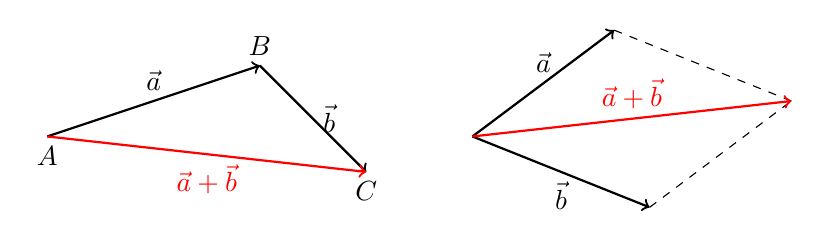
\begin{tikzpicture}[scale=0.9]
% 三角形法则
\draw[->,thick] (0,0) -- (3,1) node[midway,above] {$\vec a$};
\draw[->,thick] (3,1) -- (4.5,-0.5) node[midway,right] {$\vec b$};
\draw[->,thick,red] (0,0) -- (4.5,-0.5) node[midway,below] {$\vec a+\vec b$};
\node[below] at (0,0) {$A$};
\node[above] at (3,1) {$B$};
\node[below] at (4.5,-0.5) {$C$};
% 平行四边形法则
\draw[->,thick] (6,0) -- (8,1.5) node[midway,above] {$\vec a$};
\draw[->,thick] (6,0) -- (8.5,-1) node[midway,below] {$\vec b$};
\draw[dashed] (8,1.5) -- (10.5,0.5);
\draw[dashed] (8.5,-1) -- (10.5,0.5);
\draw[->,thick,red] (6,0) -- (10.5,0.5) node[midway,above] {$\vec a+\vec b$};
\end{tikzpicture}
\end{center}

\sectiontitle{4.3\quad 数乘向量}

\knowbox{$\lambda\vec a$：$|\lambda|>1$时方向不变、模放大；$|\lambda|<1$时缩小；$\lambda<0$时反向。}

\sectiontitle{习题4}

\begin{exercise}
\item 已知$\overrightarrow{AB}=(3,4)$（起点为原点），求$|\overrightarrow{AB}|$。
\item 化简：$\overrightarrow{AB}+\overrightarrow{BC}+\overrightarrow{CD}$
\item 已知$\vec a\;(2,1)$，$\vec b\;(1,-2)$，求$\vec a+\vec b$、$\vec a-\vec b$、$2\vec a$。
\item 在平行四边形$ABCD$中，$\overrightarrow{AB}=\vec a$，$\overrightarrow{AD}=\vec b$，用$\vec a$、$\vec b$表示$\overrightarrow{AC}$和$\overrightarrow{BD}$。
\end{exercise}

\newpage

\chaptertitle{第五章\quad 几何变换}

\sectiontitle{5.1\quad 平移}

\knowbox{
图形沿某个方向移动一定距离，形状和大小不变。\\
对应点连线平行且相等。}

\sectiontitle{5.2\quad 旋转}

\knowbox{
图形绕某一点（旋转中心）转动一定角度。\\
对应点到旋转中心的距离相等，对应点与中心连线夹角等于旋转角。\\
旋转$180^\circ$为中心对称。}

\sectiontitle{5.3\quad 轴对称}

\knowbox{
沿一条直线（对称轴）翻折，两边完全重合。\\
对称点连线被对称轴垂直平分。\\
常见轴对称图形：等腰三角形、矩形、菱形、正方形、圆。}

\sectiontitle{5.4\quad 向量在几何中的应用}

\knowbox{
利用向量法证明平行、垂直、共线问题：\\
$\vec a\parallel\vec b\Leftrightarrow\vec a=\lambda\vec b$\\
$\vec a\perp\vec b\Leftrightarrow\vec a\cdot\vec b=0$（高中阶段展开）\\
向量法解几何题的基本思路：用向量表示几何元素，利用向量运算推导。}

\sectiontitle{习题5}

\begin{exercise}
\item 将点$A(2,3)$向右平移$3$个单位再向下平移$2$个单位，得到$A'$的坐标。
\item 点$A(1,2)$绕原点逆时针旋转$90^\circ$得到$A'$，求$A'$的坐标。
\item 点$P(3,-2)$关于$x$轴、$y$轴和原点的对称点坐标各是多少？
\item 如图，$AD$是$\triangle ABC$的中线，用向量法求证：$\overrightarrow{AD}=\dfrac12(\overrightarrow{AB}+\overrightarrow{AC})$。
\item 在等腰三角形$ABC$中，$AB=AC$，$AD\perp BC$于$D$，用向量法求证$BD=DC$。
\end{exercise}

\newpage

\chaptertitle{第六章\quad 综合模型与辅助线}

\sectiontitle{6.1\quad 等高模型与等积变形}

\knowbox{
等底等高的三角形面积相等。\\
同底且顶点在与底平行的直线上移动，面积不变。\\
$A$、$B$、$C$、$D$是直线上的点，$AB=CD$，则$\triangle PAB$与$\triangle PCD$面积相等（$P$为线外一点）。}

\sectiontitle{6.2\quad 燕尾模型与共边定理}

\knowbox{
\textbf{共边定理}：若$\triangle ABC$和$\triangle DBC$有公共边$BC$，则$\dfrac{S_{\triangle ABC}}{S_{\triangle DBC}}=\dfrac{AO}{DO}$（$A$、$D$连线交$BC$于$O$）。\\
\textbf{燕尾模型}：在三角形中，通过顶点与对边上一点的连线，将三角形分成若干部分，面积之比等于对应线段之比。}

\sectiontitle{6.3\quad 常见辅助线作法}

\knowbox{
1. 遇到中线，延长一倍构造全等。\\
2. 遇到角平分线，作双垂线或截长补短。\\
3. 遇到等腰三角形，作底边上的高（三线合一）。\\
4. 遇到平行线，利用同位角、内错角相等。\\
5. 遇到中点，构造中位线（三角形中位线平行于第三边且等于其一半）。\\
6. 证明线段和差关系（如$a=b+c$），用截长补短法。}

\sectiontitle{习题6}

\begin{exercise}
\item 在$\triangle ABC$中，$D$为$BC$中点，$E$在$AD$上且$AE:ED=2:1$，求$S_{\triangle ABE}:S_{\triangle ABC}$。
\item 如图，$AB\parallel CD$，$AD$与$BC$交于$O$，$S_{\triangle AOB}=6$，$S_{\triangle COD}=24$，求$S_{\triangle AOD}$。
\item 在$\triangle ABC$中，$\angle C=90^\circ$，$AC=3$，$BC=4$，$AD$平分$\angle BAC$交$BC$于$D$，求$BD$的长。
\item 在梯形$ABCD$中，$AD\parallel BC$，$E$、$F$分别为$AB$、$CD$中点。求证：$EF\parallel AD\parallel BC$且$EF=\dfrac12(AD+BC)$。
\end{exercise}

\newpage
\sectiontitle{参考答案}

\textbf{习题1}
\begin{enumerate}
\item $\sin A=\dfrac35$，$\cos A=\dfrac45$，$\tan A=\dfrac34$
\item[(2)] (a) $1$ \qquad (b) $\dfrac12$ \qquad (c) $1$ \qquad (d) $\sqrt3$
\item $\angle A=30^\circ$，$\cos A=\dfrac{\sqrt3}{2}$
\item $AB=8$，$AC=4\sqrt3$
\end{enumerate}

\textbf{习题2}
\begin{enumerate}
\item $BC\approx5.74$，$AC\approx8.19$
\item $10\sqrt3\approx17.32$米
\item $20$海里
\item $h=10$米，$l=10\sqrt3$米
\end{enumerate}

\textbf{习题3}
\begin{enumerate}
\item $b=10\sqrt2$
\item $c=\sqrt{57}$
\item $\cos A=\dfrac57$
\item $a=\sqrt{37}$
\end{enumerate}

\textbf{习题4}
\begin{enumerate}
\item $5$
\item $\overrightarrow{AD}$
\item $\vec a+\vec b=(3,-1)$，$\vec a-\vec b=(1,3)$，$2\vec a=(4,2)$
\item $\overrightarrow{AC}=\vec a+\vec b$，$\overrightarrow{BD}=\vec b-\vec a$
\end{enumerate}

\textbf{习题5}
\begin{enumerate}
\item $A'(5,1)$
\item $A'(-2,1)$
\item 关于$x$轴$(3,2)$，关于$y$轴$(-3,-2)$，关于原点$(-3,2)$
\item $\overrightarrow{AD}=\overrightarrow{AB}+\overrightarrow{BD}=\overrightarrow{AB}+\dfrac12\overrightarrow{BC}$，$\overrightarrow{AD}=\overrightarrow{AC}-\dfrac12\overrightarrow{BC}$，相加得$\overrightarrow{AD}=\dfrac12(\overrightarrow{AB}+\overrightarrow{AC})$
\item 由$AB=AC$及$AD\perp BC$，利用向量法可得$BD=DC$
\end{enumerate}

\textbf{习题6}
\begin{enumerate}
\item $\dfrac13$
\item $12$
\item $BD=\dfrac52$
\item 连接$AF$并延长交$BC$延长线于$G$，证$\triangle ADF\cong\triangle GCF$得$CG=AD$，$EF$为$\triangle ABG$中位线，故$EF\parallel BG$且$EF=\dfrac12(BC+AD)$
\end{enumerate}

\end{document}
